The notion of an increase in complexity as an evolutionary trend has been for long part of the evolutionary thought. Advocates to this idea have used many arguments to support it. For example, adaptive reasons have been suggested, so that the increase in complexity should have been driven by natural selection (REF Bonner book).

There are however some complications to accept the existence of this trend. In the first place, before accepting the existence of such trend, we should define complexity.
More specifically, we should be able to measure the complexity of an organism in order to compare it to another one.
Furthermore, even if we find evidence of an increase of complexity in particular lineages, it would not mean that it is generalized trend (for a great review on this topic see \citep{McShea1996})


\subsection{Defining complexity}
A general definition could be "the number of component parts" of an organism\citep{McShea1996,Arthur2010}.
These "parts" might be body segments (e.g., of an insect) or genes.
%It is evident that these definitions are problematic.
It is doubtful to say that some centipede is more complex than a beetle, just based in the different number of segments they have.
Also, it is already acknowledge that there is no relation between the number of coding-genes and morphological complexity.
This lack of correspondence, sometimes referred as the "G-value paradox"
	\citep{Hahn2002},
became evident with the release of the first eukaryotic genome sequences.
Decades before, the lack of correspondence between genome size and organism complexity (or "C-value paradox") was also noted.

An alternative definition of complexity includes not only the "number of parts" but also the "interaction among parts" 
	\citep{McShea1996,Arthur2010}.
This could be illustrated with the number of gene-gene interactions (e.g., expression regulation by a transcription factor binding to a promoter region of another gene),
such that when comparing two different organisms that have same number of genes, 
one organism could be considered to be more complex than the other if the former has more gene-gene interactions than the latter.
Again this definition is disputable, as it is acknowledged that during evolution gene-gene interactions (or gene regulatory network) underlying a phenotype
can increase their complexity without affecting the phenotype itself
	\citep{Muller1999,True2001,Salazar-Ciudad2009}.

%\subsection{Complexity as number of cells}

A measure of morphological complexity that has been favoured by some authors (perhaps because of its intuitiveness), is the number of cell types that compose an organism 
	\citep{Bell1997,Bonner2004,McShea1996}.


\subsection{Complexity Increase in Evolution}

The increase in complexity in evolution has has been a topic of interest for more than a century.
Early views of evolution saw the increase in complexity as inexorable, with all the species descending from simpler ancestral forms (REF Haeckel Lamarck 1809 in McShea) and with the human species as the latest and more perfect product of the evolution of animals (REF Haeckel).


Recent views recognize that within a phylum, complexity of the species can increase or decrease.
Using the number of cell-types as complexity measure, there are clear examples of taxa that have decreased their complexity over time, specially in parasites.
Animals of the group formerly known as the "Mesozoa" are worm-like parasites of marine invertebrates.
Because of their simple morphology, these animals were thought to be "living fossils" or intermediate forms between Protozoans and Metazoans.
Now, even when they remain poorly studied animals, it is thought that they are degenerate descendants of more complex ancestors, probably some lophotrochozoan group\citep{Arthur2010}.
The Orthonectida, for example, is a phylum of parasites of marine invertebrates with only two types of cells, external ciliated and internal reproductive cells without any internal organs. 
Molecular phylogenetic analysis provided evidence that these animals are more closely related to tripoblastic animals than to protists or diplobastic taxa (REF Hanelt, 1996).
These animals most probably evolved from a more complex free living animal and decreased their morphologic complexity after they adopted a parasitic life style.

So, now is clear that there is no unique trend to increase the complexity over time, i.e., in a specific lineage, complexity might decrease, increase or stay the same (see Figure \ref{fig:Complexity_min}a).
However, if we could depict the change in complexity in all lineages (see Figure \ref{fig:Complexity_min}b), we probably would see that the range of complexity has increased over time, with the a lower limit or minimum complexity that has stayed the same and with an increase in mean and maximun (or upper limit) of complexity\citep{McShea1996,Arthur2010}.

%%%%%%%%%%%%%%%%%%%%%%%%%%%%%%%%%%%%%%%%%%%%%%%%%%%%%%%%%%%%%%%%%%%%%%%%%%%%%%%%%%%%%
\begin{figure}[t]
  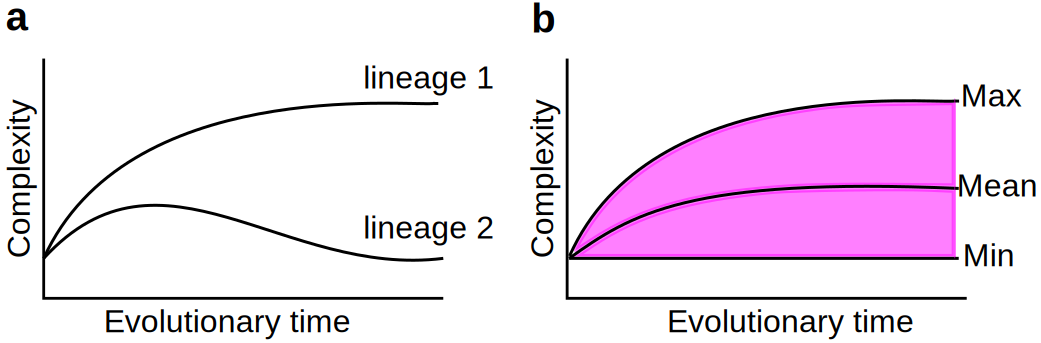
\includegraphics[width=11cm]{./Images/complexity_min.jpeg}
  \centering
  \caption{a) Two lineages with different complexity change through their evolutionary trajectories.
  b) Representation of the minimum, mean and maximum complexity of many lineages over evolutionary time in which the minimum stay constant while the mean and maximum increase.
Redrawn from \citep{Arthur2010}.
 }
  \label{fig:Complexity_min}
\end{figure}
%%%%%%%%%%%%%%%%%%%%%%%%%%%%%%%%%%%%%%%%%%%%%%%%%%%%%%%%%%%%%%%%%%%%%%%%%%%%%%%%%%%%%

\subsection{Complexity Increase in Development}

The increase in complexity in an organism during embryogenesis is probably one of the most intuitive processes of animal development. It is commonly seen even as one of its defining characteristics.
Eric H. Davidson described the progressive increase in complexity as the "essence" of development\citep{Davidson2001}.

Using the number of cell types as a proxy of morphological complexity, it can be said that during metazoan development, complexity increases as the zygote divides and differentiates into an adult with multiple cell types. 
This simple definition of complexity has its complications, as there is no clear criteria of how to define a cell type or how to determine when a new cell type has formed during development. 
For example, it could be that at the morphological level a cell seems to be undifferentiated, but when isolating it from its neighbour cells, it differentiates in an autonomous way into a specific cell type, suggesting that the cell fate was already determined without the necessity of further interactions with other cells.

\textbf{Talk about differentiation and determination?}

 
In addition, this definition does not take into account that embryos do not only get more cell types, they also organize them in specific patterns in space that could also be considered as an increase in complexity over developmental time.


%%%%%%%%%%%%%%%%%%%%%%%%%%%%%%%%%%%%%%%%%%%%%%%%%%%%%%%%%%%%%%%%%%%%%%%%%%%%%%%%%%%%%
%\clearpage
\begin{mdframed}[style=boxstyle,frametitle={Box1. On the similarity of complexity patterns between Evolution and Development}]\label{Box1:Haeckel&vonBaer}

The connection between the increase in complexity during development and evolutionary time it has been largely discussed.
Haeckel was one of the first who made explicit hypothesis about the connection between the development and evolutionary patterns.
In what is known as Haeckel's "Biogenetic Law", he described development (or ontogeny), as a brief summary of the slow and long phylogeny (REF Haeckel 1903 in Richardson 2002).
In his hypothesis, a "higher" organism would pass through a series of conserved developmental stages that represent ancestral forms. This view is also known as the "recapitulation theory".

Karl Ernst von Baer, an Estonian naturalist, also formulated his own hypotheses, known as von Baer's laws. He stated that general characteristics develop before special characteristics (first law) and, opposed to Haeckel, that the embryo of a "higher" animal never resembles the adult of another animal form, but only his embryo (fourth law). 

Apart from the differences in the "recapitulation" view of Haeckel and von Baer\citep{Richardson2002}, they disagreed in the acceptance of evolution. 
Haeckel's view was an evolutionary one, while von Baer's was not. Curiously, von Baer's arguments were used by Darwin in its "Origin of species" to support common ancestry and therefore, evolution.

Now is evident that any of these hypotheses can be considered "laws", as they are not universal. They only apply to some characters, stages and levels of phylogenetic inclusiveness \citep{Richardson2002}. Nevertheless, both Haeckel and von Baer work represented the foundations of the comparative embryology field, which is turn the basis of the modern evolutionary developmental biology (evo-devo).
	\nomenclature{Evo-devo}{Evolutionary Developmental Biology}
\end{mdframed}
%%%%%%%%%%%%%%%%%%%%%%%%%%%%%%%%%%%%%%%%%%%%%%%%%%%%%%%%%%%%%%%%%%%%%%%%%%%%%%%%%%%%%


	

\subsection{Complexity at the molecular level}

It seems expectable that the increase in complexity over time, whether evolutionary or developmental, should be associated with an underlying increase in complexity at the molecular level \citep{Arthur2010}, following the reasoning that:
i) in order to achieve an increased morphological complexity in an advanced embryological stage, new cell types should form.
ii) Different cell-types are characterized by the differential expression of genes.
iii) Therefore, the more cell-types an organism is formed of, more different combinations of expressed genes has to have (with the gene regulatory complexity this must entail).

Indeed, development is often visualized at the molecular level as an 

At the level of gene expression it seems also clear that the embryo becomes progressively compartmentalized over time and space. In spite of this intuitiveness, there is again

increased in complexity as:

- cis-regulatory regions GRN (davidson)

- miRNA

- nothing about spatial or statistical approach like our disparity measure
